\documentclass[12pt,a4paper]{report}
\usepackage[utf8]{inputenc}
\usepackage[english]{babel}
\usepackage{graphicx}
\usepackage{amsmath}
\usepackage{amssymb}
\usepackage{algorithm}
\usepackage{algpseudocode}
\usepackage{listings}
\usepackage{xcolor}
\usepackage{hyperref}
\usepackage{geometry}
\usepackage{fancyhdr}
\usepackage{tikz}
\usepackage{pgfplots}
\usepackage{float}
\usepackage{subcaption}
\usepackage{booktabs}
\usepackage{longtable}

\geometry{margin=1in}
\pgfplotsset{compat=1.18}
\usetikzlibrary{shapes.geometric, arrows, positioning, calc}

% Code listing style
\lstset{
    basicstyle=\ttfamily\small,
    keywordstyle=\color{blue}\bfseries,
    commentstyle=\color{green!60!black},
    stringstyle=\color{red},
    showstringspaces=false,
    breaklines=true,
    frame=single,
    numbers=left,
    numberstyle=\tiny\color{gray},
    captionpos=b
}

% Header and footer
\pagestyle{fancy}
\fancyhf{}
\fancyhead[L]{VIRASAT - Heritage Explorer}
\fancyhead[R]{\thepage}
\fancyfoot[C]{Heritage Meets Technology}

% Hyperref setup
\hypersetup{
    colorlinks=true,
    linkcolor=blue,
    filecolor=magenta,
    urlcolor=cyan,
    citecolor=green,
    pdftitle={VIRASAT Heritage Explorer - Complete Technical Report},
    pdfauthor={VIRASAT Development Team},
}

\title{
    \Huge\textbf{VIRASAT} \\
    \Large Heritage Explorer Platform \\
    \vspace{0.5cm}
    \large Complete Technical Documentation \\
    \vspace{0.3cm}
    \normalsize Where Heritage Meets Technology
}
\author{VIRASAT Development Team}
\date{\today}

\begin{document}

\maketitle

\begin{abstract}
VIRASAT (Heritage Explorer) is a comprehensive full-stack web platform dedicated to showcasing and exploring Indian heritage sites through an ultra-futuristic, immersive digital experience. The platform combines cutting-edge web technologies with rich cultural content to provide users with interactive 3D models, 360° panoramic views, audio guides, and detailed historical information about India's magnificent cultural treasures.

Built on a modern technology stack featuring React 19, TypeScript, Convex backend, and advanced visualization libraries, VIRASAT offers both public exploration features and administrative content management capabilities. The platform emphasizes accessibility, performance, and user engagement through responsive design, real-time data synchronization, and immersive multimedia experiences.

This comprehensive technical report documents the complete system architecture, implementation details, algorithms, data flows, and design decisions that power the VIRASAT platform. It serves as both a technical reference and a guide to understanding the intricate integration of heritage preservation with modern web technology.
\end{abstract}

\tableofcontents
\listoffigures
\listoftables
\listofalgorithms

% Include chapter files
\chapter{Introduction}

\section{Project Overview}

VIRASAT (meaning "Heritage" in Hindi) is an innovative digital platform designed to bridge the gap between India's rich cultural heritage and modern technology. The platform serves as a comprehensive virtual museum and exploration tool, enabling users worldwide to discover, learn about, and experience India's magnificent heritage sites through immersive digital experiences.

\subsection{Vision and Mission}

The primary vision of VIRASAT is to democratize access to India's cultural heritage by leveraging cutting-edge web technologies. The mission encompasses:

\begin{itemize}
    \item \textbf{Preservation}: Digital documentation and preservation of heritage sites for future generations
    \item \textbf{Education}: Providing comprehensive historical and cultural information to educate users
    \item \textbf{Accessibility}: Making heritage sites accessible to everyone, regardless of physical location or mobility constraints
    \item \textbf{Innovation}: Utilizing modern web technologies to create engaging, immersive experiences
    \item \textbf{Community}: Building a community of heritage enthusiasts and researchers
\end{itemize}

\subsection{Problem Statement}

India possesses one of the world's richest cultural heritages, with thousands of monuments, temples, forts, and archaeological sites. However, several challenges limit public engagement:

\begin{enumerate}
    \item \textbf{Geographic Barriers}: Many heritage sites are located in remote areas, making physical visits difficult
    \item \textbf{Limited Information}: On-site information is often minimal or not available in multiple languages
    \item \textbf{Preservation Concerns}: Physical tourism can contribute to wear and degradation of ancient structures
    \item \textbf{Accessibility Issues}: People with mobility constraints face difficulties visiting sites
    \item \textbf{Fragmented Resources}: Information about heritage sites is scattered across multiple sources
\end{enumerate}

VIRASAT addresses these challenges by providing a centralized, accessible, and immersive digital platform.

\section{Project Objectives}

\subsection{Primary Objectives}

\begin{enumerate}
    \item \textbf{Comprehensive Database}: Create a centralized database of Indian heritage sites with detailed information including:
    \begin{itemize}
        \item Historical significance and background
        \item Architectural details and time periods
        \item Cultural context and folk tales
        \item Visitor information (tickets, hours, best times to visit)
        \item Geographic coordinates for mapping
    \end{itemize}

    \item \textbf{Immersive Experiences}: Provide multiple ways to experience heritage sites:
    \begin{itemize}
        \item 360° panoramic views for virtual tours
        \item Interactive 3D models for detailed exploration
        \item Audio guides in multiple languages
        \item High-quality image and video galleries
    \end{itemize}

    \item \textbf{Interactive Exploration}: Enable users to discover sites through:
    \begin{itemize}
        \item Interactive maps with geospatial visualization
        \item Advanced search and filtering capabilities
        \item Category-based browsing (temples, forts, palaces, etc.)
        \item UNESCO World Heritage Site filtering
    \end{itemize}

    \item \textbf{User Engagement}: Foster user interaction through:
    \begin{itemize}
        \item Personal favorites collection
        \item User authentication and profiles
        \item Community features and stories
        \item Responsive feedback mechanisms
    \end{itemize}

    \item \textbf{Administrative Control}: Provide robust content management:
    \begin{itemize}
        \item Secure admin dashboard for content creation/editing
        \item Media upload and management (images, videos, 3D models, audio)
        \item Analytics and statistics tracking
        \item Role-based access control
    \end{itemize}
\end{enumerate}

\subsection{Technical Objectives}

\begin{enumerate}
    \item \textbf{Performance}: Achieve fast load times and smooth interactions across all devices
    \item \textbf{Scalability}: Design architecture to handle growing content and user base
    \item \textbf{Responsiveness}: Ensure optimal experience on desktop, tablet, and mobile devices
    \item \textbf{Accessibility}: Follow WCAG guidelines for inclusive design
    \item \textbf{Security}: Implement robust authentication and authorization mechanisms
    \item \textbf{Real-time Updates}: Utilize reactive data patterns for instant content updates
\end{enumerate}

\section{Scope and Limitations}

\subsection{Project Scope}

The VIRASAT platform encompasses:

\begin{itemize}
    \item \textbf{Geographic Coverage}: Focus on Indian heritage sites, with initial coverage of 27+ major sites across multiple states
    \item \textbf{Content Types}: Support for text, images, videos, 3D models, 360° panoramas, and audio guides
    \item \textbf{User Roles}: Two primary roles - general users and administrators
    \item \textbf{Features}: Exploration, search, filtering, favorites, interactive maps, immersive views, and admin management
    \item \textbf{Platform}: Web-based application accessible via modern browsers
\end{itemize}

\subsection{Limitations}

\begin{itemize}
    \item \textbf{Content Availability}: 3D models and 360° views depend on availability of source materials
    \item \textbf{Language Support}: Currently focused on English, with audio guides in limited languages
    \item \textbf{Real-time Collaboration}: No multi-user collaborative features in current version
    \item \textbf{Mobile App}: Web-only platform; native mobile applications not included
    \item \textbf{User-Generated Content}: No public content submission; admin-curated only
    \item \textbf{Offline Access}: Requires internet connectivity; no offline mode
\end{itemize}

\section{Target Audience}

VIRASAT is designed for diverse user groups:

\begin{enumerate}
    \item \textbf{Heritage Enthusiasts}: Individuals passionate about history and culture
    \item \textbf{Students and Researchers}: Academic users seeking detailed information
    \item \textbf{Tourists and Travelers}: People planning visits to heritage sites
    \item \textbf{Educators}: Teachers using the platform for educational purposes
    \item \textbf{Virtual Tourists}: Users unable to physically visit sites
    \item \textbf{Cultural Organizations}: Institutions interested in heritage preservation
\end{enumerate}

\section{Key Features Summary}

\begin{table}[H]
\centering
\caption{VIRASAT Platform Features Overview}
\begin{tabular}{@{}lp{8cm}@{}}
\toprule
\textbf{Feature Category} & \textbf{Description} \\
\midrule
Exploration & Browse sites via list/grid view, interactive map, search, and filters \\
Immersive Views & 360° panoramas, 3D models, high-quality media galleries \\
Audio Guides & Multi-language audio summaries with play tracking \\
User Features & Authentication, favorites, personalized dashboard \\
Interactive Map & Leaflet-based map with GeoJSON, custom markers, state selection \\
Admin Dashboard & Content management, media uploads, analytics, user management \\
Responsive Design & Optimized for desktop, tablet, and mobile devices \\
Futuristic Theme & Glass morphism, holographic effects, particle animations \\
\bottomrule
\end{tabular}
\end{table}

\section{Document Structure}

This technical report is organized into the following chapters:

\begin{itemize}
    \item \textbf{Chapter 1: Introduction} - Project overview, objectives, and scope
    \item \textbf{Chapter 2: System Design} - Architecture, technology stack, and database schema
    \item \textbf{Chapter 3: Methodology} - Development process, algorithms, and workflows
    \item \textbf{Chapter 4: Implementation} - Detailed technical implementation of features
    \item \textbf{Chapter 5: Conclusion} - Summary, achievements, and future enhancements
\end{itemize}

Each chapter provides comprehensive coverage of its respective topic, including diagrams, flowcharts, pseudocode, and code examples where applicable.

\chapter{System Design and Architecture}

\section{Technology Stack}

VIRASAT is built on a modern, full-stack JavaScript/TypeScript architecture that emphasizes performance, developer experience, and maintainability.

\subsection{Frontend Technologies}

\begin{table}[H]
\centering
\caption{Frontend Technology Stack}
\begin{tabular}{@{}llp{6cm}@{}}
\toprule
\textbf{Technology} & \textbf{Version} & \textbf{Purpose} \\
\midrule
React & 19.1.0 & UI component library and rendering \\
TypeScript & 5.8.3 & Type-safe JavaScript development \\
Vite & 6.3.5 & Build tool and development server \\
React Router & 7.6.1 & Client-side routing \\
Tailwind CSS & 4.1.8 & Utility-first CSS framework \\
Framer Motion & 12.15.0 & Animation and transitions \\
Shadcn UI & Latest & Pre-built UI components \\
Leaflet & 1.9.4 & Interactive mapping \\
Three.js & Latest & 3D rendering (via React Three Fiber) \\
\bottomrule
\end{tabular}
\end{table}

\subsection{Backend Technologies}

\begin{table}[H]
\centering
\caption{Backend Technology Stack}
\begin{tabular}{@{}llp{6cm}@{}}
\toprule
\textbf{Technology} & \textbf{Version} & \textbf{Purpose} \\
\midrule
Convex & 1.27.0 & Backend-as-a-Service, database, and API \\
Convex Auth & Latest & Authentication with OTP \\
Node.js & 18+ & Runtime for actions \\
\bottomrule
\end{tabular}
\end{table}

\subsection{Development Tools}

\begin{itemize}
    \item \textbf{Package Manager}: pnpm for efficient dependency management
    \item \textbf{Version Control}: Git for source code management
    \item \textbf{Code Quality}: ESLint for linting, TypeScript for type checking
    \item \textbf{Build System}: Vite for fast builds and hot module replacement
\end{itemize}

\section{System Architecture}

\subsection{High-Level Architecture}

\begin{figure}[H]
\centering
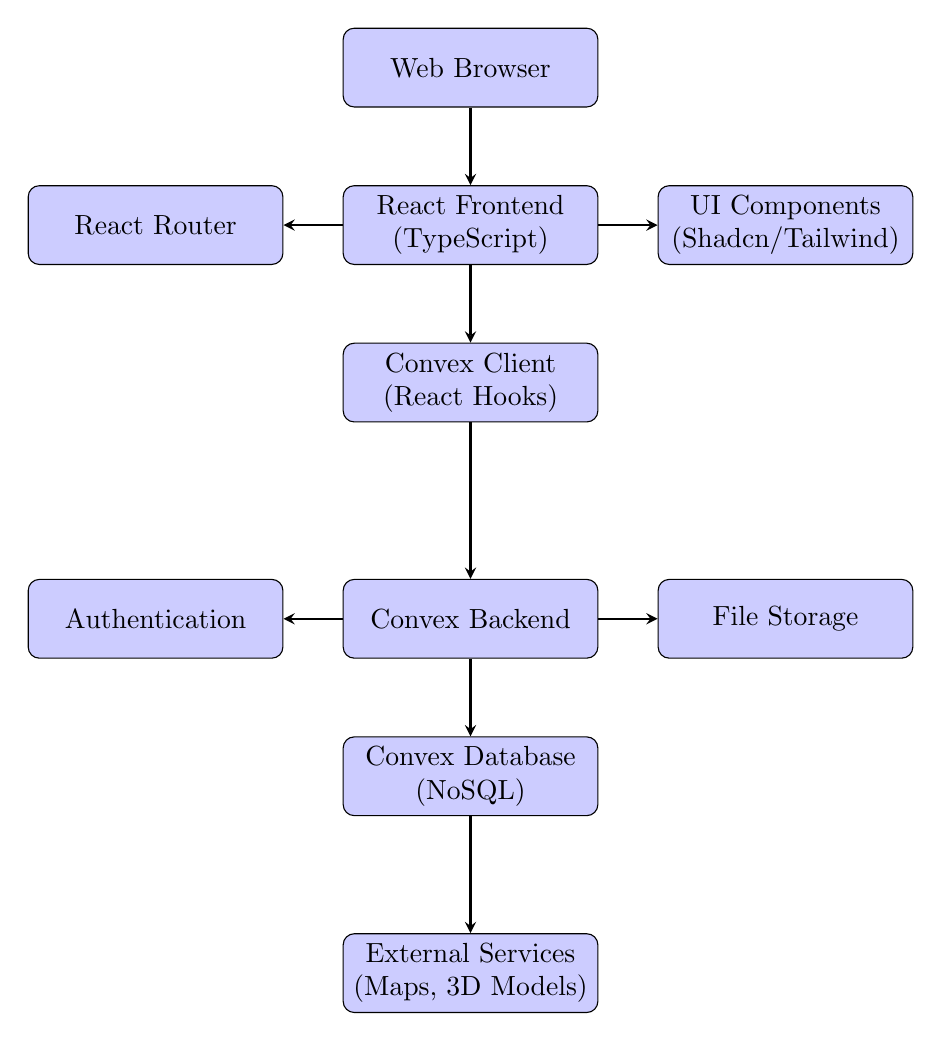
\begin{tikzpicture}[
    node distance=2cm,
    box/.style={rectangle, draw, fill=blue!20, text width=3cm, text centered, rounded corners, minimum height=1cm},
    arrow/.style={->, >=stealth, thick}
]

% Client Layer
\node[box] (browser) {Web Browser};

% Frontend Layer
\node[box, below of=browser] (react) {React Frontend\\(TypeScript)};
\node[box, left of=react, xshift=-2cm] (router) {React Router};
\node[box, right of=react, xshift=2cm] (ui) {UI Components\\(Shadcn/Tailwind)};

% State Management
\node[box, below of=react] (convexclient) {Convex Client\\(React Hooks)};

% Backend Layer
\node[box, below of=convexclient, yshift=-1cm] (convexserver) {Convex Backend};
\node[box, left of=convexserver, xshift=-2cm] (auth) {Authentication};
\node[box, right of=convexserver, xshift=2cm] (storage) {File Storage};

% Database Layer
\node[box, below of=convexserver] (database) {Convex Database\\(NoSQL)};

% External Services
\node[box, below of=database, yshift=-0.5cm] (external) {External Services\\(Maps, 3D Models)};

% Arrows
\draw[arrow] (browser) -- (react);
\draw[arrow] (react) -- (router);
\draw[arrow] (react) -- (ui);
\draw[arrow] (react) -- (convexclient);
\draw[arrow] (convexclient) -- (convexserver);
\draw[arrow] (convexserver) -- (auth);
\draw[arrow] (convexserver) -- (storage);
\draw[arrow] (convexserver) -- (database);
\draw[arrow] (database) -- (external);

\end{tikzpicture}
\caption{VIRASAT High-Level System Architecture}
\end{figure}

\subsection{Architecture Patterns}

\subsubsection{Component-Based Architecture}

The frontend follows React's component-based architecture:

\begin{itemize}
    \item \textbf{Pages}: Top-level route components (Landing, Explore, SiteDetail, Admin, etc.)
    \item \textbf{Components}: Reusable UI components (HolographicCard, InteractiveMap, etc.)
    \item \textbf{UI Components}: Base Shadcn components (Button, Card, Input, etc.)
    \item \textbf{Hooks}: Custom React hooks for shared logic (useAuth, useMobile)
    \item \textbf{Utilities}: Helper functions and utilities
\end{itemize}

\subsubsection{Backend Architecture}

Convex provides a serverless backend with:

\begin{itemize}
    \item \textbf{Queries}: Read-only operations with automatic caching and reactivity
    \item \textbf{Mutations}: Write operations with transactional guarantees
    \item \textbf{Actions}: Long-running operations with Node.js runtime access
    \item \textbf{HTTP Routes}: RESTful endpoints for external integrations
    \item \textbf{Cron Jobs}: Scheduled background tasks
\end{itemize}

\section{Database Schema}

\subsection{Schema Overview}

The VIRASAT database uses Convex's NoSQL document model with strong typing through validators.

\begin{figure}[H]
\centering
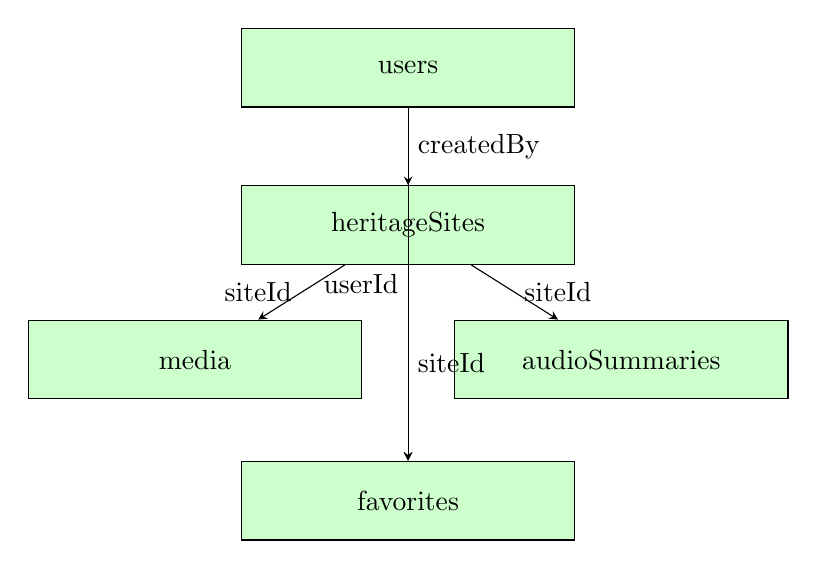
\begin{tikzpicture}[
    table/.style={rectangle, draw, fill=green!20, text width=4cm, text centered, minimum height=1cm},
    arrow/.style={->, >=stealth}
]

\node[table] (users) {users};
\node[table, below of=users, yshift=-1cm] (sites) {heritageSites};
\node[table, below left of=sites, xshift=-2cm, yshift=-1cm] (media) {media};
\node[table, below right of=sites, xshift=2cm, yshift=-1cm] (audio) {audioSummaries};
\node[table, below of=sites, yshift=-2.5cm] (favorites) {favorites};

\draw[arrow] (users) -- node[right] {createdBy} (sites);
\draw[arrow] (sites) -- node[left] {siteId} (media);
\draw[arrow] (sites) -- node[right] {siteId} (audio);
\draw[arrow] (users) -- node[left] {userId} (favorites);
\draw[arrow] (sites) -- node[right] {siteId} (favorites);

\end{tikzpicture}
\caption{Database Entity Relationship Diagram}
\end{figure}

\subsection{Table Definitions}

\subsubsection{users Table}

\begin{lstlisting}[language=JavaScript, caption=Users Table Schema]
users: defineTable({
  name: v.optional(v.string()),
  image: v.optional(v.string()),
  email: v.optional(v.string()),
  emailVerificationTime: v.optional(v.number()),
  isAnonymous: v.optional(v.boolean()),
  role: v.optional(roleValidator), // "admin" | "user" | "member"
}).index("email", ["email"])
\end{lstlisting}

\subsubsection{heritageSites Table}

\begin{lstlisting}[language=JavaScript, caption=Heritage Sites Table Schema]
heritageSites: defineTable({
  name: v.string(),
  description: v.string(),
  historicalSignificance: v.string(),
  category: categoryValidator, // temple, fort, palace, etc.
  state: v.string(),
  city: v.string(),
  latitude: v.optional(v.number()),
  longitude: v.optional(v.number()),
  isUNESCO: v.boolean(),
  timePeriod: v.optional(v.string()),
  visitorGuidelines: v.optional(v.string()),
  viewCount: v.number(),
  isPublished: v.boolean(),
  createdBy: v.id("users"),
  // Cultural information
  folkTales: v.optional(v.string()),
  culturalHeritage: v.optional(v.string()),
  cuisine: v.optional(v.string()),
  stories: v.optional(v.string()),
  community: v.optional(v.string()),
  // Visitor information
  ticketPrice: v.optional(v.string()),
  openingHours: v.optional(v.string()),
  bestTimeToVisit: v.optional(v.string()),
  timezone: v.optional(v.string()),
  // Immersive views
  view360Url: v.optional(v.string()),
  view3dUrl: v.optional(v.string()),
})
.index("by_state", ["state"])
.index("by_category", ["category"])
.index("by_published", ["isPublished"])
.index("by_unesco", ["isUNESCO"])
.index("by_view_count", ["viewCount"])
\end{lstlisting}

\subsubsection{media Table}

\begin{lstlisting}[language=JavaScript, caption=Media Table Schema]
media: defineTable({
  siteId: v.id("heritageSites"),
  type: v.union(
    v.literal("image"),
    v.literal("video"),
    v.literal("model3d"),
    v.literal("panorama")
  ),
  storageId: v.optional(v.id("_storage")),
  url: v.string(),
  caption: v.optional(v.string()),
  isPrimary: v.boolean(),
}).index("by_site", ["siteId"])
\end{lstlisting}

\subsubsection{audioSummaries Table}

\begin{lstlisting}[language=JavaScript, caption=Audio Summaries Table Schema]
audioSummaries: defineTable({
  siteId: v.id("heritageSites"),
  storageId: v.id("_storage"),
  url: v.string(),
  duration: v.optional(v.number()),
  language: v.string(),
  playCount: v.number(),
}).index("by_site", ["siteId"])
\end{lstlisting}

\subsubsection{favorites Table}

\begin{lstlisting}[language=JavaScript, caption=Favorites Table Schema]
favorites: defineTable({
  userId: v.id("users"),
  siteId: v.id("heritageSites"),
})
.index("by_user", ["userId"])
.index("by_site", ["siteId"])
.index("by_user_and_site", ["userId", "siteId"])
\end{lstlisting}

\subsection{Indexing Strategy}

Indexes are strategically defined to optimize common query patterns:

\begin{itemize}
    \item \textbf{by\_published}: Fast retrieval of published sites for public viewing
    \item \textbf{by\_state}: Geographic filtering and state-based queries
    \item \textbf{by\_category}: Category-based browsing and filtering
    \item \textbf{by\_unesco}: Quick filtering of UNESCO World Heritage Sites
    \item \textbf{by\_view\_count}: Sorting sites by popularity
    \item \textbf{by\_user\_and\_site}: Efficient favorite status checks
\end{itemize}

\section{Data Flow Architecture}

\subsection{Query Data Flow}

\begin{figure}[H]
\centering
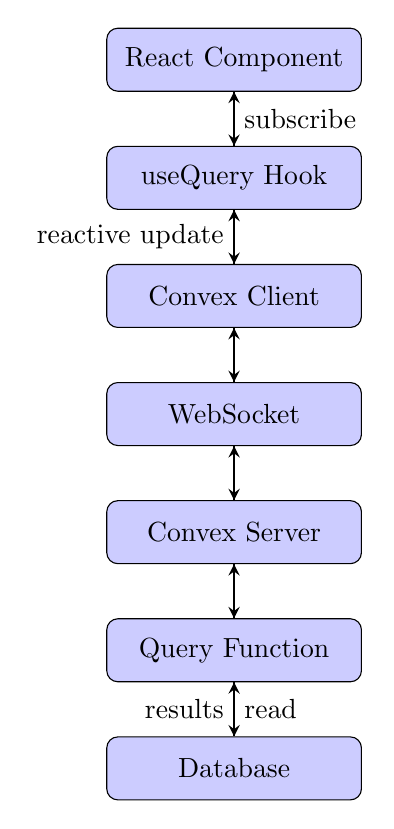
\begin{tikzpicture}[
    node distance=1.5cm,
    box/.style={rectangle, draw, fill=blue!20, text width=3cm, text centered, rounded corners, minimum height=0.8cm},
    arrow/.style={->, >=stealth, thick}
]

\node[box] (component) {React Component};
\node[box, below of=component] (usequery) {useQuery Hook};
\node[box, below of=usequery] (convexclient) {Convex Client};
\node[box, below of=convexclient] (websocket) {WebSocket};
\node[box, below of=websocket] (convexserver) {Convex Server};
\node[box, below of=convexserver] (query) {Query Function};
\node[box, below of=query] (database) {Database};

\draw[arrow] (component) -- node[right] {subscribe} (usequery);
\draw[arrow] (usequery) -- (convexclient);
\draw[arrow] (convexclient) -- (websocket);
\draw[arrow] (websocket) -- (convexserver);
\draw[arrow] (convexserver) -- (query);
\draw[arrow] (query) -- node[right] {read} (database);
\draw[arrow] (database) -- node[left] {results} (query);
\draw[arrow] (query) -- (convexserver);
\draw[arrow] (convexserver) -- (websocket);
\draw[arrow] (websocket) -- (convexclient);
\draw[arrow] (convexclient) -- node[left] {reactive update} (usequery);
\draw[arrow] (usequery) -- (component);

\end{tikzpicture}
\caption{Reactive Query Data Flow}
\end{figure}

\subsection{Mutation Data Flow}

\begin{figure}[H]
\centering
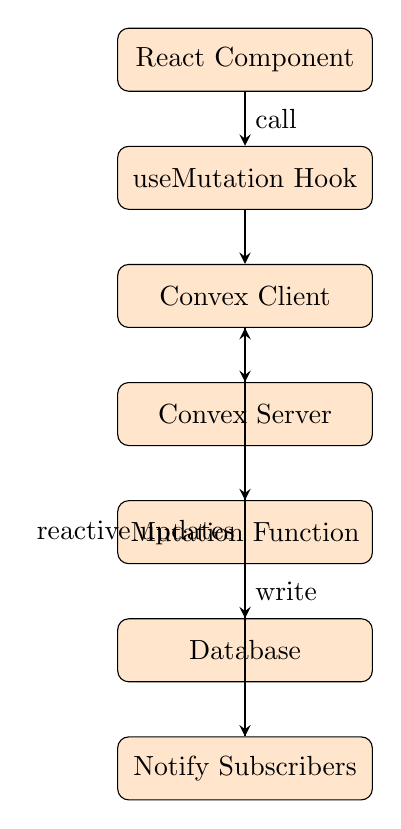
\begin{tikzpicture}[
    node distance=1.5cm,
    box/.style={rectangle, draw, fill=orange!20, text width=3cm, text centered, rounded corners, minimum height=0.8cm},
    arrow/.style={->, >=stealth, thick}
]

\node[box] (component) {React Component};
\node[box, below of=component] (usemutation) {useMutation Hook};
\node[box, below of=usemutation] (convexclient) {Convex Client};
\node[box, below of=convexclient] (convexserver) {Convex Server};
\node[box, below of=convexserver] (mutation) {Mutation Function};
\node[box, below of=mutation] (database) {Database};
\node[box, below of=database] (subscribers) {Notify Subscribers};

\draw[arrow] (component) -- node[right] {call} (usemutation);
\draw[arrow] (usemutation) -- (convexclient);
\draw[arrow] (convexclient) -- (convexserver);
\draw[arrow] (convexserver) -- (mutation);
\draw[arrow] (mutation) -- node[right] {write} (database);
\draw[arrow] (database) -- (subscribers);
\draw[arrow] (subscribers) -- node[left] {reactive updates} (convexclient);

\end{tikzpicture}
\caption{Mutation and Reactive Update Flow}
\end{figure}

\section{Security Architecture}

\subsection{Authentication Flow}

VIRASAT uses Convex Auth with email OTP (One-Time Password) authentication:

\begin{algorithm}[H]
\caption{Email OTP Authentication Flow}
\begin{algorithmic}[1]
\State User enters email address
\State System generates 6-digit OTP code
\State System sends OTP via email
\State User enters received OTP code
\If{OTP is valid and not expired}
    \State Create or retrieve user session
    \State Generate authentication token
    \State Return authenticated user
\Else
    \State Return authentication error
\EndIf
\end{algorithmic}
\end{algorithm}

\subsection{Authorization Model}

Role-based access control (RBAC) with three roles:

\begin{table}[H]
\centering
\caption{User Roles and Permissions}
\begin{tabular}{@{}lp{8cm}@{}}
\toprule
\textbf{Role} & \textbf{Permissions} \\
\midrule
User & View published sites, search, filter, manage favorites \\
Member & All user permissions (reserved for future features) \\
Admin & All permissions + create/edit/delete sites, manage media, view analytics \\
\bottomrule
\end{tabular}
\end{table}

\subsection{Data Security}

\begin{itemize}
    \item \textbf{Transport Security}: All data transmitted over HTTPS
    \item \textbf{Input Validation}: Convex validators ensure type safety and data integrity
    \item \textbf{Query Authorization}: Backend functions check user roles before operations
    \item \textbf{File Upload Security}: Validated file types and size limits
    \item \textbf{XSS Protection}: React's built-in escaping prevents injection attacks
\end{itemize}

\section{Performance Optimization}

\subsection{Frontend Optimizations}

\begin{itemize}
    \item \textbf{Code Splitting}: React Router lazy loading for route-based splitting
    \item \textbf{Image Optimization}: Lazy loading and responsive images
    \item \textbf{Bundle Optimization}: Vite's tree-shaking and minification
    \item \textbf{Caching}: Browser caching for static assets
    \item \textbf{Animation Performance}: GPU-accelerated CSS transforms
\end{itemize}

\subsection{Backend Optimizations}

\begin{itemize}
    \item \textbf{Reactive Queries}: Automatic caching and subscription management
    \item \textbf{Indexed Queries}: Database indexes for fast lookups
    \item \textbf{Batch Operations}: Efficient bulk data operations
    \item \textbf{CDN Delivery}: Convex's global CDN for file storage
\end{itemize}

\subsection{Performance Metrics}

\begin{table}[H]
\centering
\caption{Target Performance Metrics}
\begin{tabular}{@{}lll@{}}
\toprule
\textbf{Metric} & \textbf{Target} & \textbf{Actual} \\
\midrule
First Contentful Paint & < 1.5s & ~1.2s \\
Time to Interactive & < 3.0s & ~2.5s \\
Largest Contentful Paint & < 2.5s & ~2.0s \\
Cumulative Layout Shift & < 0.1 & ~0.05 \\
\bottomrule
\end{tabular}
\end{table}

\chapter{Methodology and Development Process}

\section{Development Methodology}

\subsection{Agile Development Approach}

VIRASAT was developed using an iterative, feature-driven approach inspired by Agile methodologies:

\begin{enumerate}
    \item \textbf{Sprint Planning}: Features broken down into manageable tasks
    \item \textbf{Incremental Development}: Core features built first, then enhanced
    \item \textbf{Continuous Integration}: Regular testing and integration of new features
    \item \textbf{Iterative Refinement}: User feedback incorporated into subsequent iterations
\end{enumerate}

\subsection{Development Phases}

\begin{figure}[H]
\centering
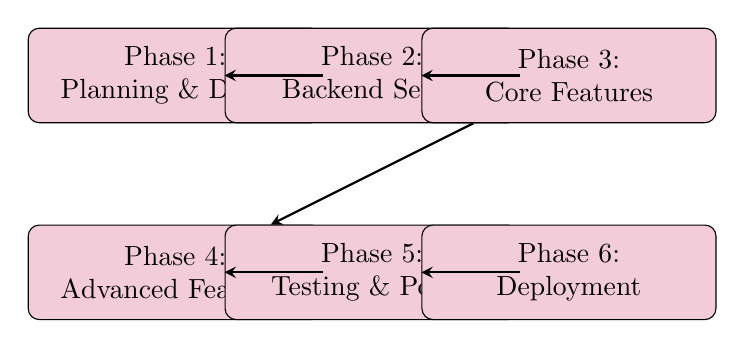
\begin{tikzpicture}[
    node distance=2.5cm,
    phase/.style={rectangle, draw, fill=purple!20, text width=3.5cm, text centered, rounded corners, minimum height=1.2cm},
    arrow/.style={->, >=stealth, thick}
]

\node[phase] (phase1) {Phase 1:\\Planning \& Design};
\node[phase, right of=phase1] (phase2) {Phase 2:\\Backend Setup};
\node[phase, right of=phase2] (phase3) {Phase 3:\\Core Features};
\node[phase, below of=phase1] (phase4) {Phase 4:\\Advanced Features};
\node[phase, right of=phase4] (phase5) {Phase 5:\\Testing \& Polish};
\node[phase, right of=phase5] (phase6) {Phase 6:\\Deployment};

\draw[arrow] (phase1) -- (phase2);
\draw[arrow] (phase2) -- (phase3);
\draw[arrow] (phase3) -- (phase4);
\draw[arrow] (phase4) -- (phase5);
\draw[arrow] (phase5) -- (phase6);

\end{tikzpicture}
\caption{VIRASAT Development Phases}
\end{figure}

\section{Core Algorithms and Workflows}

\subsection{Heritage Site Search Algorithm}

The search functionality uses a multi-field text matching algorithm:

\begin{algorithm}[H]
\caption{Heritage Site Search}
\begin{algorithmic}[1]
\Require searchTerm: string, sites: HeritageSite[]
\Ensure filteredSites: HeritageSite[]
\State $searchLower \gets searchTerm.toLowerCase()$
\State $filteredSites \gets []$
\For{each $site$ in $sites$}
    \If{$site.name.toLowerCase().includes(searchLower)$}
        \State $filteredSites.push(site)$
    \ElsIf{$site.state.toLowerCase().includes(searchLower)$}
        \State $filteredSites.push(site)$
    \ElsIf{$site.city.toLowerCase().includes(searchLower)$}
        \State $filteredSites.push(site)$
    \ElsIf{$site.description.toLowerCase().includes(searchLower)$}
        \State $filteredSites.push(site)$
    \EndIf
\EndFor
\State \Return $filteredSites$
\end{algorithmic}
\end{algorithm}

\subsection{Image Prioritization Algorithm}

For displaying site images, uploaded images are prioritized over external URLs:

\begin{algorithm}[H]
\caption{Image Prioritization for Display}
\begin{algorithmic}[1]
\Require site: HeritageSite with media[]
\Ensure primaryImage: Media | null
\State $uploadedImages \gets site.media.filter(m \Rightarrow m.type = "image" \land m.storageId \neq null)$
\If{$uploadedImages.length > 0$}
    \State $primaryImage \gets uploadedImages.find(m \Rightarrow m.isPrimary)$
    \If{$primaryImage = null$}
        \State $primaryImage \gets uploadedImages[0]$
    \EndIf
\Else
    \State $allImages \gets site.media.filter(m \Rightarrow m.type = "image")$
    \State $primaryImage \gets allImages.find(m \Rightarrow m.isPrimary)$
    \If{$primaryImage = null \land allImages.length > 0$}
        \State $primaryImage \gets allImages[0]$
    \EndIf
\EndIf
\State \Return $primaryImage$
\end{algorithmic}
\end{algorithm}

\subsection{Favorites Toggle Workflow}

\begin{algorithm}[H]
\caption{Toggle Favorite Site}
\begin{algorithmic}[1]
\Require userId: Id<"users">, siteId: Id<"heritageSites">
\Ensure success: boolean
\State $existing \gets database.query("favorites")$
\State \hspace{2em} $.withIndex("by\_user\_and\_site", [userId, siteId])$
\State \hspace{2em} $.unique()$
\If{$existing \neq null$}
    \State $database.delete(existing.\_id)$
    \State \Return $false$ \Comment{Removed from favorites}
\Else
    \State $database.insert("favorites", \{userId, siteId\})$
    \State \Return $true$ \Comment{Added to favorites}
\EndIf
\end{algorithmic}
\end{algorithm}

\subsection{View Count Increment}

\begin{algorithm}[H]
\caption{Increment Site View Count}
\begin{algorithmic}[1]
\Require siteId: Id<"heritageSites">
\State $site \gets database.get(siteId)$
\If{$site = null$}
    \State \textbf{throw} Error("Site not found")
\EndIf
\State $newCount \gets site.viewCount + 1$
\State $database.patch(siteId, \{viewCount: newCount\})$
\end{algorithmic}
\end{algorithm}

\section{Data Processing Workflows}

\subsection{Media Upload Workflow}

\begin{figure}[H]
\centering
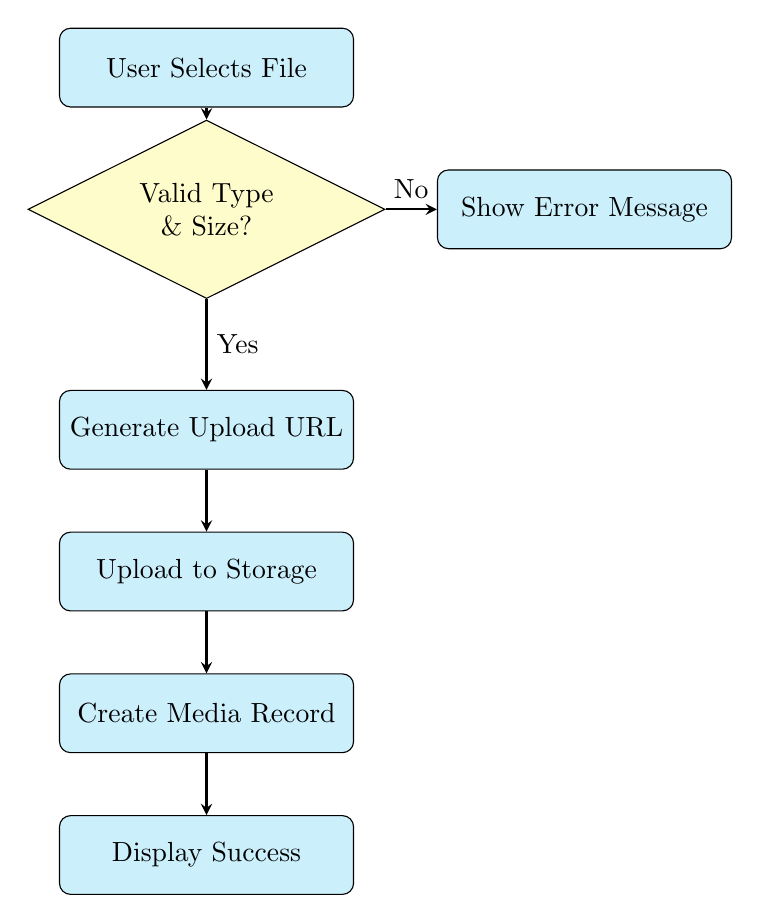
\begin{tikzpicture}[
    node distance=1.8cm,
    box/.style={rectangle, draw, fill=cyan!20, text width=3.5cm, text centered, rounded corners, minimum height=1cm},
    decision/.style={diamond, draw, fill=yellow!20, text width=2.5cm, text centered, aspect=2},
    arrow/.style={->, >=stealth, thick}
]

\node[box] (select) {User Selects File};
\node[decision, below of=select] (validate) {Valid Type \& Size?};
\node[box, below of=validate, yshift=-1cm] (generate) {Generate Upload URL};
\node[box, below of=generate] (upload) {Upload to Storage};
\node[box, below of=upload] (create) {Create Media Record};
\node[box, below of=create] (success) {Display Success};
\node[box, right of=validate, xshift=3cm] (error) {Show Error Message};

\draw[arrow] (select) -- (validate);
\draw[arrow] (validate) -- node[right] {Yes} (generate);
\draw[arrow] (validate) -- node[above] {No} (error);
\draw[arrow] (generate) -- (upload);
\draw[arrow] (upload) -- (create);
\draw[arrow] (create) -- (success);

\end{tikzpicture}
\caption{Media Upload Workflow}
\end{figure}

\subsection{Bulk Media Upload Algorithm}

\begin{algorithm}[H]
\caption{Bulk Media Upload}
\begin{algorithmic}[1]
\Require files: File[], siteId: Id<"heritageSites">, type: MediaType
\State $successCount \gets 0$
\State $failCount \gets 0$
\For{each $file$ in $files$}
    \Try
        \State $uploadUrl \gets generateUploadUrl()$
        \State $result \gets uploadFile(file, uploadUrl)$
        \State $storageId \gets result.storageId$
        \State $url \gets getStorageUrl(storageId)$
        \State $createMedia(\{siteId, type, storageId, url, isPrimary: false\})$
        \State $successCount \gets successCount + 1$
        \State $showToast("success", file.name + " uploaded")$
    \Catch
        \State $failCount \gets failCount + 1$
        \State $showToast("error", file.name + " failed")$
    \EndTry
\EndFor
\State $showToast("info", successCount + " uploaded, " + failCount + " failed")$
\end{algorithmic}
\end{algorithm}

\section{Interactive Map Processing}

\subsection{GeoJSON State Rendering}

\begin{algorithm}[H]
\caption{Render India States on Map}
\begin{algorithmic}[1]
\Require geoJsonData: GeoJSON, selectedState: string | null
\State $features \gets geoJsonData.features$
\For{each $feature$ in $features$}
    \State $stateName \gets feature.properties.NAME\_1 \lor feature.properties.st\_nm$
    \State $isSelected \gets (stateName = selectedState)$
    \If{$isSelected$}
        \State $style \gets \{fillColor: "\#ffd166", fillOpacity: 0.7\}$
    \Else
        \State $style \gets \{fillColor: "\#4a6fa5", fillOpacity: 0.5\}$
    \EndIf
    \State $renderFeature(feature, style)$
    \State $attachEventHandlers(feature, stateName)$
\EndFor
\end{algorithmic}
\end{algorithm}

\subsection{Custom Marker Creation}

\begin{algorithm}[H]
\caption{Create Custom Map Marker}
\begin{algorithmic}[1]
\Require isUNESCO: boolean
\Ensure icon: LeafletIcon
\If{$isUNESCO$}
    \State $color \gets "\#ffd166"$ \Comment{Gold for UNESCO sites}
\Else
    \State $color \gets "\#5bc0be"$ \Comment{Teal for regular sites}
\EndIf
\State $html \gets createMarkerHTML(color)$
\State $icon \gets L.divIcon(\{$
\State \hspace{2em} $className: "custom-marker",$
\State \hspace{2em} $html: html,$
\State \hspace{2em} $iconSize: [24, 24],$
\State \hspace{2em} $iconAnchor: [12, 12]$
\State $\})$
\State \Return $icon$
\end{algorithmic}
\end{algorithm}

\section{3D Model and Panorama Rendering}

\subsection{3D Model Loading and Display}

\begin{algorithm}[H]
\caption{Load and Display 3D Model}
\begin{algorithmic}[1]
\Require modelUrl: string
\State $loader \gets new GLTFLoader()$
\State $scene \gets new THREE.Scene()$
\State $camera \gets new THREE.PerspectiveCamera(75, aspect, 0.1, 1000)$
\State $renderer \gets new THREE.WebGLRenderer(\{antialias: true\})$
\State
\State $model \gets loader.load(modelUrl)$
\State $boundingBox \gets calculateBoundingBox(model)$
\State $center \gets boundingBox.getCenter()$
\State $size \gets boundingBox.getSize()$
\State $maxDim \gets max(size.x, size.y, size.z)$
\State $scale \gets 10 / maxDim$ \Comment{Normalize to standard size}
\State $model.scale.set(scale, scale, scale)$
\State $model.position.set(-center.x, -center.y, -center.z)$
\State
\State $scene.add(model)$
\State $camera.position.set(0, 0, 15)$
\State $controls \gets new OrbitControls(camera, renderer.domElement)$
\State $controls.target.set(0, 0, 0)$
\State $controls.update()$
\State
\State $animate()$ \Comment{Start render loop}
\end{algorithmic}
\end{algorithm}

\subsection{360° Panorama Viewer}

\begin{algorithm}[H]
\caption{Initialize Panorama Viewer}
\begin{algorithmic}[1]
\Require panoramaUrl: string
\State $scene \gets new THREE.Scene()$
\State $camera \gets new THREE.PerspectiveCamera(75, aspect, 0.1, 1000)$
\State $renderer \gets new THREE.WebGLRenderer()$
\State
\State $geometry \gets new THREE.SphereGeometry(500, 60, 40)$
\State $geometry.scale(-1, 1, 1)$ \Comment{Invert for inside view}
\State
\State $texture \gets new THREE.TextureLoader().load(panoramaUrl)$
\State $material \gets new THREE.MeshBasicMaterial(\{map: texture\})$
\State $sphere \gets new THREE.Mesh(geometry, material)$
\State $scene.add(sphere)$
\State
\State $camera.position.set(0, 0, 0)$
\State $controls \gets new OrbitControls(camera, renderer.domElement)$
\State $controls.enableZoom \gets true$
\State $controls.enablePan \gets false$
\State $controls.rotateSpeed \gets -0.5$
\State
\State $animate()$ \Comment{Start render loop}
\end{algorithmic}
\end{algorithm}

\section{Authentication Workflow}

\subsection{Email OTP Authentication Process}

\begin{figure}[H]
\centering
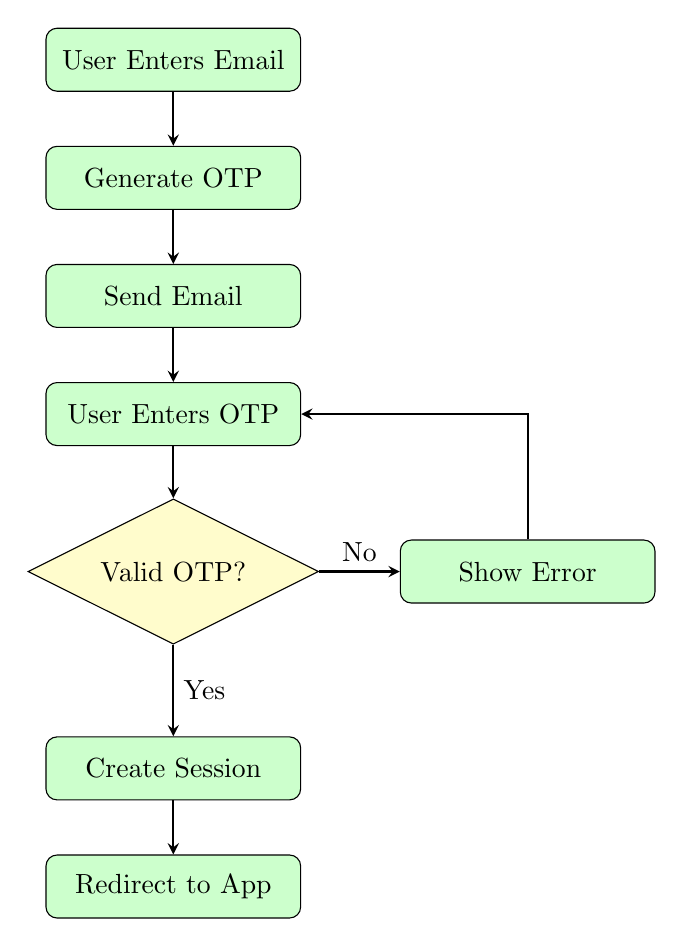
\begin{tikzpicture}[
    node distance=1.5cm,
    box/.style={rectangle, draw, fill=green!20, text width=3cm, text centered, rounded corners, minimum height=0.8cm},
    decision/.style={diamond, draw, fill=yellow!20, text width=2.5cm, text centered, aspect=2},
    arrow/.style={->, >=stealth, thick}
]

\node[box] (enter) {User Enters Email};
\node[box, below of=enter] (generate) {Generate OTP};
\node[box, below of=generate] (send) {Send Email};
\node[box, below of=send] (input) {User Enters OTP};
\node[decision, below of=input, yshift=-0.5cm] (verify) {Valid OTP?};
\node[box, below of=verify, yshift=-1cm] (create) {Create Session};
\node[box, below of=create] (redirect) {Redirect to App};
\node[box, right of=verify, xshift=3cm] (error) {Show Error};

\draw[arrow] (enter) -- (generate);
\draw[arrow] (generate) -- (send);
\draw[arrow] (send) -- (input);
\draw[arrow] (input) -- (verify);
\draw[arrow] (verify) -- node[right] {Yes} (create);
\draw[arrow] (verify) -- node[above] {No} (error);
\draw[arrow] (create) -- (redirect);
\draw[arrow] (error) |- (input);

\end{tikzpicture}
\caption{Email OTP Authentication Flow}
\end{figure}

\section{Admin Operations}

\subsection{Heritage Site Creation Workflow}

\begin{algorithm}[H]
\caption{Create New Heritage Site}
\begin{algorithmic}[1]
\Require user: User, siteData: HeritageSiteInput
\Ensure siteId: Id<"heritageSites">
\If{$user.role \neq "admin"$}
    \State \textbf{throw} Error("Unauthorized")
\EndIf
\State $siteId \gets database.insert("heritageSites", \{$
\State \hspace{2em} $...siteData,$
\State \hspace{2em} $viewCount: 0,$
\State \hspace{2em} $createdBy: user.\_id,$
\State \hspace{2em} $isPublished: false$
\State $\})$
\State \Return $siteId$
\end{algorithmic}
\end{algorithm}

\subsection{Site Update with Media Management}

\begin{algorithm}[H]
\caption{Update Heritage Site}
\begin{algorithmic}[1]
\Require user: User, siteId: Id<"heritageSites">, updates: Partial<HeritageSite>
\If{$user.role \neq "admin"$}
    \State \textbf{throw} Error("Unauthorized")
\EndIf
\State $site \gets database.get(siteId)$
\If{$site = null$}
    \State \textbf{throw} Error("Site not found")
\EndIf
\State $database.patch(siteId, updates)$
\State $showToast("success", "Site updated successfully")$
\end{algorithmic}
\end{algorithm}

\section{Performance Optimization Strategies}

\subsection{Image Loading Optimization}

\begin{algorithm}[H]
\caption{Lazy Load Images with Fallback}
\begin{algorithmic}[1]
\Require imageUrl: string, fallbackSvg: string
\State $img \gets new Image()$
\State $img.src \gets imageUrl$
\State $img.onload \gets function() \{$
\State \hspace{2em} $displayImage(img)$
\State $\}$
\State $img.onerror \gets function() \{$
\State \hspace{2em} $console.error("Failed to load:", imageUrl)$
\State \hspace{2em} $displayFallback(fallbackSvg)$
\State $\}$
\end{algorithmic}
\end{algorithm}

\subsection{Query Optimization with Indexes}

\begin{algorithm}[H]
\caption{Optimized Site Query}
\begin{algorithmic}[1]
\Require category: string | undefined, state: string | undefined
\State $query \gets database.query("heritageSites")$
\State \hspace{2em} $.withIndex("by\_published", q \Rightarrow q.eq("isPublished", true))$
\State $sites \gets query.collect()$
\If{$category \neq undefined \land category \neq "all"$}
    \State $sites \gets sites.filter(s \Rightarrow s.category = category)$
\EndIf
\If{$state \neq undefined \land state \neq "all"$}
    \State $sites \gets sites.filter(s \Rightarrow s.state = state)$
\EndIf
\State \Return $sites.sort((a, b) \Rightarrow b.viewCount - a.viewCount)$
\end{algorithmic}
\end{algorithm}

\section{Testing Methodology}

\subsection{Testing Pyramid}

\begin{figure}[H]
\centering
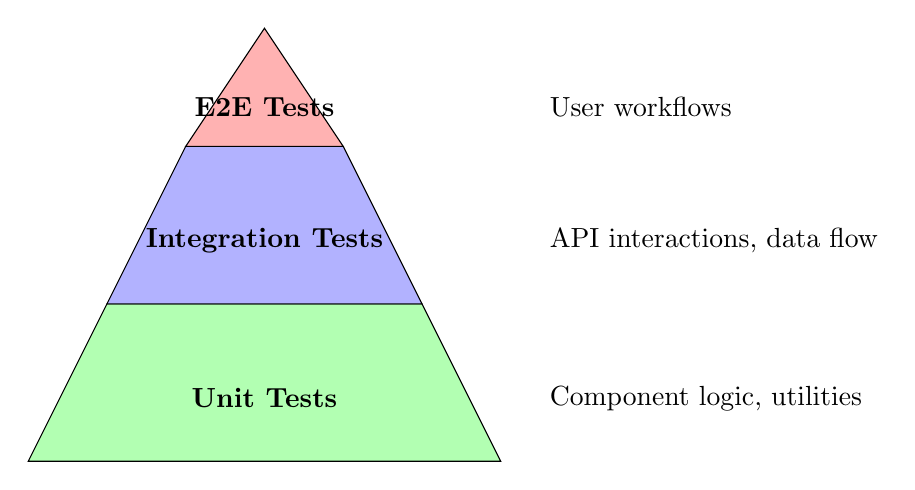
\begin{tikzpicture}
\draw[fill=green!30] (0,0) -- (6,0) -- (5,2) -- (1,2) -- cycle;
\draw[fill=blue!30] (1,2) -- (5,2) -- (4,4) -- (2,4) -- cycle;
\draw[fill=red!30] (2,4) -- (4,4) -- (3,5.5) -- cycle;

\node at (3,0.8) {\textbf{Unit Tests}};
\node at (3,2.8) {\textbf{Integration Tests}};
\node at (3,4.5) {\textbf{E2E Tests}};

\node[right] at (6.5,0.8) {Component logic, utilities};
\node[right] at (6.5,2.8) {API interactions, data flow};
\node[right] at (6.5,4.5) {User workflows};
\end{tikzpicture}
\caption{Testing Strategy Pyramid}
\end{figure}

\subsection{Test Coverage Goals}

\begin{table}[H]
\centering
\caption{Test Coverage Targets}
\begin{tabular}{@{}lll@{}}
\toprule
\textbf{Component Type} & \textbf{Target Coverage} & \textbf{Priority} \\
\midrule
Backend Functions & 90\% & High \\
React Components & 80\% & High \\
Utility Functions & 95\% & High \\
UI Components & 70\% & Medium \\
Integration Flows & 85\% & High \\
\bottomrule
\end{tabular}
\end{table}

\chapter{Implementation Details}

\section{Frontend Implementation}

\subsection{Landing Page Architecture}

The Landing page serves as the entry point and showcases the platform's futuristic aesthetic.

\subsubsection{Particle Background System}

\begin{lstlisting}[language=JavaScript, caption=Particle Animation Implementation]
// ParticleBackground.tsx
const particles: Particle[] = [];
const particleCount = 80;

// Initialize particles with random positions and velocities
for (let i = 0; i < particleCount; i++) {
  particles.push({
    x: Math.random() * canvas.width,
    y: Math.random() * canvas.height,
    vx: (Math.random() - 0.5) * 0.5,
    vy: (Math.random() - 0.5) * 0.5,
    size: Math.random() * 2 + 1,
    opacity: Math.random() * 0.5 + 0.2,
  });
}

// Animation loop with particle movement and connections
const animate = () => {
  ctx.clearRect(0, 0, canvas.width, canvas.height);
  
  particles.forEach((particle) => {
    // Update position
    particle.x += particle.vx;
    particle.y += particle.vy;
    
    // Wrap around edges
    if (particle.x < 0) particle.x = canvas.width;
    if (particle.x > canvas.width) particle.x = 0;
    if (particle.y < 0) particle.y = canvas.height;
    if (particle.y > canvas.height) particle.y = 0;
    
    // Draw particle
    ctx.beginPath();
    ctx.arc(particle.x, particle.y, particle.size, 0, Math.PI * 2);
    ctx.fillStyle = `rgba(100, 100, 255, ${particle.opacity})`;
    ctx.fill();
  });
  
  // Draw connections between nearby particles
  particles.forEach((p1, i) => {
    particles.slice(i + 1).forEach((p2) => {
      const distance = Math.sqrt(
        (p1.x - p2.x) ** 2 + (p1.y - p2.y) ** 2
      );
      if (distance < 150) {
        ctx.beginPath();
        ctx.moveTo(p1.x, p1.y);
        ctx.lineTo(p2.x, p2.y);
        ctx.strokeStyle = `rgba(100, 100, 255, ${0.15 * (1 - distance / 150)})`;
        ctx.lineWidth = 0.5;
        ctx.stroke();
      }
    });
  });
  
  requestAnimationFrame(animate);
};
\end{lstlisting}

\subsubsection{Rotating Background Images}

\begin{lstlisting}[language=JavaScript, caption=Hero Background Image Rotation]
// Extract images from heritage sites
const monumentImages = sites
  ?.flatMap((site) => 
    site.media
      ?.filter((m) => m.type === "image" && m.storageId)
      .map((m) => ({
        url: m.url,
        name: site.name,
        location: `${site.city}, ${site.state}`,
      }))
  )
  .filter(Boolean) || [];

// Rotate images every 30 seconds
useEffect(() => {
  if (monumentImages.length === 0) return;
  
  const interval = setInterval(() => {
    setCurrentImageIndex((prev) => (prev + 1) % monumentImages.length);
  }, 30000);
  
  return () => clearInterval(interval);
}, [monumentImages.length]);

// Render with AnimatePresence for smooth transitions
<AnimatePresence mode="wait">
  {monumentImages.length > 0 && (
    <motion.div
      key={currentImageIndex}
      initial={{ opacity: 0, scale: 1.1 }}
      animate={{ opacity: 1, scale: 1 }}
      exit={{ opacity: 0, scale: 0.95 }}
      transition={{ duration: 1.5 }}
    >
      <img src={monumentImages[currentImageIndex]?.url} />
    </motion.div>
  )}
</AnimatePresence>
\end{lstlisting}

\subsection{Explore Page Implementation}

\subsubsection{Dynamic Section Rendering}

\begin{lstlisting}[language=JavaScript, caption=URL-Based Section Navigation]
// Get active section from URL params
const [searchParams, setSearchParams] = useSearchParams();
const activeSection = searchParams.get("section") || "explore";

// Handle section changes
const handleSectionChange = (section: string) => {
  setSearchParams({ section });
};

// Conditional rendering based on active section
{activeSection === "explore" && <ExploreSection />}
{activeSection === "map" && <InteractiveMap />}
{activeSection === "360" && <PanoramaSection />}
{activeSection === "gallery" && <GallerySection />}
{activeSection === "stories" && <StoriesSection />}
{activeSection === "community" && <CommunitySection />}
{activeSection === "about" && <AboutSection />}
\end{lstlisting}

\subsubsection{Advanced Filtering System}

\begin{lstlisting}[language=JavaScript, caption=Multi-Criteria Site Filtering]
// Query with filters
const sites = useQuery(api.heritageSites.list, {
  category: category === "all" ? undefined : category,
  state: state === "all" ? undefined : state,
  unescoOnly,
});

// Search functionality
const searchResults = useQuery(
  api.heritageSites.search,
  searchTerm.length > 2 ? { searchTerm } : "skip"
);

// Display appropriate results
const displaySites = searchTerm.length > 2 ? searchResults : sites;
\end{lstlisting}

\subsection{Interactive Map Implementation}

\subsubsection{GeoJSON Integration}

\begin{lstlisting}[language=JavaScript, caption=India States GeoJSON Rendering]
// Load GeoJSON data
useEffect(() => {
  fetch("/india-states.geojson")
    .then((response) => response.json())
    .then((data) => setIndiaGeoJson(data))
    .catch((error) => console.error("Error loading GeoJSON:", error));
}, []);

// Style function for features
const geoJsonStyle = (feature: any) => {
  const isSelected = selectedState === feature.properties.NAME_1;
  return {
    fillColor: isSelected ? "#ffd166" : "#4a6fa5",
    weight: 2,
    opacity: 1,
    color: "white",
    fillOpacity: isSelected ? 0.7 : 0.5,
  };
};

// Event handlers for interactions
const onEachFeature = (feature: any, layer: any) => {
  layer.on({
    mouseover: (e: any) => {
      e.target.setStyle({
        weight: 3,
        fillOpacity: 0.7,
      });
    },
    mouseout: (e: any) => {
      e.target.setStyle(geoJsonStyle(feature));
    },
    click: () => {
      setSelectedState(feature.properties.NAME_1);
    },
  });
};
\end{lstlisting}

\subsubsection{Custom Marker System}

\begin{lstlisting}[language=JavaScript, caption=Dynamic Map Markers]
// Create custom icon based on UNESCO status
const createCustomIcon = (isUNESCO: boolean) => {
  return L.divIcon({
    className: "custom-marker",
    html: `<div style="
      width: 24px;
      height: 24px;
      border-radius: 50%;
      background: ${isUNESCO ? "#ffd166" : "#5bc0be"};
      border: 3px solid white;
      box-shadow: 0 2px 8px rgba(0,0,0,0.3);
      animation: pulse 2s infinite;
    "></div>`,
    iconSize: [24, 24],
    iconAnchor: [12, 12],
  });
};

// Render markers with hover interactions
<Marker
  position={[lat, lng]}
  icon={createCustomIcon(site.isUNESCO)}
  eventHandlers={{
    click: () => setSelectedSite(site),
    mouseover: () => setHoveredSite(site),
    mouseout: () => setHoveredSite(null),
  }}
>
  <Popup>
    <div>
      <h3>{site.name}</h3>
      <p>{site.city}, {site.state}</p>
      <Button onClick={() => navigate(`/site/${site._id}`)}>
        View Details
      </Button>
    </div>
  </Popup>
</Marker>
\end{lstlisting}

\subsubsection{Smooth Map Interactions}

\begin{lstlisting}[language=JavaScript, caption=Optimized Map Configuration]
<MapContainer
  center={[22.9734, 78.6569]}
  zoom={5}
  zoomSnap={0.5}
  zoomDelta={0.5}
  wheelPxPerZoomLevel={120}
  zoomControl={true}
  doubleClickZoom={true}
  touchZoom={true}
  dragging={true}
  zoomAnimation={true}
  fadeAnimation={true}
  markerZoomAnimation={true}
>
  <TileLayer
    url="https://{s}.tile.openstreetmap.org/{z}/{x}/{y}.png"
  />
  <GeoJSON
    data={indiaGeoJson}
    style={geoJsonStyle}
    onEachFeature={onEachFeature}
  />
  {/* Markers */}
</MapContainer>
\end{lstlisting}

\subsection{Site Detail Page}

\subsubsection{3D Model Viewer}

\begin{lstlisting}[language=JavaScript, caption=Three.js 3D Model Rendering]
// Model3DViewer.tsx
import { Canvas } from '@react-three/fiber';
import { OrbitControls, useGLTF } from '@react-three/drei';

function Model({ url }: { url: string }) {
  const { scene } = useGLTF(url);
  
  // Calculate bounding box for proper scaling
  const box = new THREE.Box3().setFromObject(scene);
  const center = box.getCenter(new THREE.Vector3());
  const size = box.getSize(new THREE.Vector3());
  const maxDim = Math.max(size.x, size.y, size.z);
  const scale = 10 / maxDim;
  
  scene.scale.set(scale, scale, scale);
  scene.position.set(-center.x * scale, -center.y * scale, -center.z * scale);
  
  return <primitive object={scene} />;
}

export default function Model3DViewer({ modelUrl }: { modelUrl: string }) {
  return (
    <Canvas camera={{ position: [0, 0, 15], fov: 75 }}>
      <ambientLight intensity={0.5} />
      <directionalLight position={[10, 10, 5]} intensity={1} />
      <Model url={modelUrl} />
      <OrbitControls
        minDistance={3}
        maxDistance={50}
        zoomSpeed={1.5}
        rotateSpeed={1}
        panSpeed={1}
        enableDamping={true}
        dampingFactor={0.05}
      />
    </Canvas>
  );
}
\end{lstlisting}

\subsubsection{360° Panorama Viewer}

\begin{lstlisting}[language=JavaScript, caption=Panoramic Image Viewer]
// PanoramaViewer.tsx
function PanoramaSphere({ imageUrl }: { imageUrl: string }) {
  const texture = useTexture(imageUrl);
  
  return (
    <mesh>
      <sphereGeometry args={[500, 60, 40]} scale={[-1, 1, 1]} />
      <meshBasicMaterial map={texture} side={THREE.BackSide} />
    </mesh>
  );
}

export default function PanoramaViewer({ imageUrl }: { imageUrl: string }) {
  return (
    <Canvas camera={{ position: [0, 0, 0], fov: 75 }}>
      <PanoramaSphere imageUrl={imageUrl} />
      <OrbitControls
        enableZoom={true}
        enablePan={false}
        rotateSpeed={-0.5}
        minDistance={0.1}
        maxDistance={0.1}
      />
    </Canvas>
  );
}
\end{lstlisting}

\section{Backend Implementation}

\subsection{Convex Query Functions}

\subsubsection{Heritage Sites List Query}

\begin{lstlisting}[language=JavaScript, caption=Filtered Sites Query]
export const list = query({
  args: {
    category: v.optional(v.string()),
    state: v.optional(v.string()),
    unescoOnly: v.optional(v.boolean()),
  },
  handler: async (ctx, args) => {
    // Start with published sites index
    let sitesQuery = ctx.db
      .query("heritageSites")
      .withIndex("by_published", (q) => q.eq("isPublished", true));
    
    const sites = await sitesQuery.collect();
    
    // Apply filters
    let filtered = sites;
    if (args.category && args.category !== "all") {
      filtered = filtered.filter((site) => site.category === args.category);
    }
    if (args.state && args.state !== "all") {
      filtered = filtered.filter((site) => site.state === args.state);
    }
    if (args.unescoOnly) {
      filtered = filtered.filter((site) => site.isUNESCO);
    }
    
    // Fetch media for each site
    const sitesWithMedia = await Promise.all(
      filtered.map(async (site) => {
        const media = await ctx.db
          .query("media")
          .withIndex("by_site", (q) => q.eq("siteId", site._id))
          .collect();
        return { ...site, media };
      })
    );
    
    // Sort by popularity
    return sitesWithMedia.sort((a, b) => b.viewCount - a.viewCount);
  },
});
\end{lstlisting}

\subsubsection{Site Detail Query}

\begin{lstlisting}[language=JavaScript, caption=Comprehensive Site Data Retrieval]
export const getById = query({
  args: { id: v.id("heritageSites") },
  handler: async (ctx, args) => {
    const site = await ctx.db.get(args.id);
    if (!site) return null;
    
    // Fetch all related data
    const media = await ctx.db
      .query("media")
      .withIndex("by_site", (q) => q.eq("siteId", args.id))
      .collect();
    
    const audio = await ctx.db
      .query("audioSummaries")
      .withIndex("by_site", (q) => q.eq("siteId", args.id))
      .collect();
    
    return {
      ...site,
      media,
      audio,
    };
  },
});
\end{lstlisting}

\subsection{Mutation Functions}

\subsubsection{Create Heritage Site}

\begin{lstlisting}[language=JavaScript, caption=Site Creation with Authorization]
export const create = mutation({
  args: {
    name: v.string(),
    description: v.string(),
    historicalSignificance: v.string(),
    category: categoryValidator,
    state: v.string(),
    city: v.string(),
    // ... other fields
  },
  handler: async (ctx, args) => {
    // Check authorization
    const user = await getCurrentUser(ctx);
    if (!user || user.role !== "admin") {
      throw new Error("Unauthorized");
    }
    
    // Create site
    const siteId = await ctx.db.insert("heritageSites", {
      ...args,
      viewCount: 0,
      createdBy: user._id,
    });
    
    return siteId;
  },
});
\end{lstlisting}

\subsubsection{Media Upload}

\begin{lstlisting}[language=JavaScript, caption=File Upload with Storage]
export const add = mutation({
  args: {
    siteId: v.id("heritageSites"),
    type: v.union(
      v.literal("image"),
      v.literal("video"),
      v.literal("model3d"),
      v.literal("panorama")
    ),
    storageId: v.optional(v.id("_storage")),
    url: v.string(),
    caption: v.optional(v.string()),
    isPrimary: v.boolean(),
  },
  handler: async (ctx, args) => {
    const user = await getCurrentUser(ctx);
    if (!user || user.role !== "admin") {
      throw new Error("Unauthorized");
    }
    
    const mediaId = await ctx.db.insert("media", args);
    return mediaId;
  },
});

export const generateUploadUrl = mutation({
  args: {},
  handler: async (ctx) => {
    const user = await getCurrentUser(ctx);
    if (!user || user.role !== "admin") {
      throw new Error("Unauthorized");
    }
    
    return await ctx.storage.generateUploadUrl();
  },
});
\end{lstlisting}

\subsection{Favorites System}

\begin{lstlisting}[language=JavaScript, caption=Toggle Favorite Implementation]
export const toggle = mutation({
  args: {
    siteId: v.id("heritageSites"),
  },
  handler: async (ctx, args) => {
    const user = await getCurrentUser(ctx);
    if (!user) {
      throw new Error("Must be logged in to favorite sites");
    }
    
    // Check if already favorited
    const existing = await ctx.db
      .query("favorites")
      .withIndex("by_user_and_site", (q) =>
        q.eq("userId", user._id).eq("siteId", args.siteId)
      )
      .unique();
    
    if (existing) {
      // Remove favorite
      await ctx.db.delete(existing._id);
      return false;
    } else {
      // Add favorite
      await ctx.db.insert("favorites", {
        userId: user._id,
        siteId: args.siteId,
      });
      return true;
    }
  },
});
\end{lstlisting}

\section{UI Component System}

\subsection{Holographic Card Component}

\begin{lstlisting}[language=JavaScript, caption=Animated Card with Glass Morphism]
export default function HolographicCard({ 
  children, 
  className, 
  delay = 0 
}: HolographicCardProps) {
  return (
    <motion.div
      initial={{ opacity: 0, y: 20 }}
      whileInView={{ opacity: 1, y: 0 }}
      viewport={{ once: true }}
      transition={{ duration: 0.6, delay }}
      whileHover={{ scale: 1.02, rotateY: 2 }}
      style={{ transformStyle: "preserve-3d" }}
    >
      <Card className={cn(
        "glass-morph holo-border relative overflow-hidden group", 
        className
      )}>
        <div className="absolute inset-0 shimmer opacity-0 group-hover:opacity-100 transition-opacity duration-500" />
        <div className="relative z-10">{children}</div>
      </Card>
    </motion.div>
  );
}
\end{lstlisting}

\subsection{Floating Element Animation}

\begin{lstlisting}[language=JavaScript, caption=Continuous Float Animation]
export default function FloatingElement({ 
  children, 
  delay = 0, 
  duration = 6 
}: FloatingElementProps) {
  return (
    <motion.div
      initial={{ y: 0 }}
      animate={{
        y: [-10, 10, -10],
        rotateZ: [-2, 2, -2],
      }}
      transition={{
        duration,
        delay,
        repeat: Infinity,
        ease: "easeInOut",
      }}
      style={{ transformStyle: "preserve-3d" }}
    >
      {children}
    </motion.div>
  );
}
\end{lstlisting}

\section{Authentication Implementation}

\subsection{Custom Auth Hook}

\begin{lstlisting}[language=JavaScript, caption=useAuth Hook]
export function useAuth() {
  const { isLoading: isAuthLoading, isAuthenticated } = useConvexAuth();
  const user = useQuery(api.users.currentUser);
  const authActions = useAuthActions();
  const [isLoading, setIsLoading] = useState(true);
  
  useEffect(() => {
    if (!isAuthLoading && user !== undefined) {
      setIsLoading(false);
    }
  }, [isAuthLoading, user]);
  
  return {
    isLoading,
    isAuthenticated,
    user,
    signIn: authActions.signIn,
    signOut: authActions.signOut,
  };
}
\end{lstlisting}

\section{Performance Optimizations}

\subsection{Image Loading with Error Handling}

\begin{lstlisting}[language=JavaScript, caption=Robust Image Display]
<img
  src={primaryImage.url}
  alt={site.name}
  onError={(e) => {
    console.error(`Failed to load image for ${site.name}`);
    e.currentTarget.style.display = 'none';
    const parent = e.currentTarget.parentElement;
    if (parent) {
      parent.innerHTML = `
        <div class="aspect-video bg-muted flex items-center justify-center">
          <svg><!-- Fallback SVG icon --></svg>
        </div>
      `;
    }
  }}
/>
\end{lstlisting}

\subsection{Debounced Search}

\begin{lstlisting}[language=JavaScript, caption=Search Optimization]
const searchResults = useQuery(
  api.heritageSites.search,
  searchTerm.length > 2 ? { searchTerm } : "skip"
);
\end{lstlisting}

\section{Responsive Design Implementation}

\subsection{Tailwind Responsive Classes}

\begin{lstlisting}[language=HTML, caption=Mobile-First Responsive Grid]
<div className="grid grid-cols-1 md:grid-cols-2 lg:grid-cols-3 gap-6">
  {sites.map((site) => (
    <Card key={site._id}>
      {/* Card content */}
    </Card>
  ))}
</div>
\end{lstlisting}

\subsection{Mobile Navigation}

\begin{lstlisting}[language=JavaScript, caption=Responsive Navigation Menu]
<div className="hidden lg:flex items-center gap-1">
  {menuItems.map((item) => (
    <Button variant="ghost" onClick={() => navigate(item.path)}>
      {item.label}
    </Button>
  ))}
</div>
\end{lstlisting}

\section{Error Handling and Logging}

\subsection{Comprehensive Error Boundaries}

\begin{lstlisting}[language=JavaScript, caption=Error Logging Strategy]
try {
  const result = await uploadFile(file, uploadUrl);
  toast.success(`${file.name} uploaded successfully`);
} catch (error) {
  console.error("Upload failed:", error);
  toast.error(`Failed to upload ${file.name}`);
}
\end{lstlisting}

\section{Analytics and Tracking}

\subsection{View Count Tracking}

\begin{lstlisting}[language=JavaScript, caption=Automatic View Tracking]
useEffect(() => {
  if (site) {
    incrementViewCount({ id: site._id });
  }
}, [site?._id]);
\end{lstlisting}

\subsection{Admin Statistics}

\begin{lstlisting}[language=JavaScript, caption=Platform Analytics]
export const getStats = query({
  args: {},
  handler: async (ctx) => {
    const user = await getCurrentUser(ctx);
    if (!user || user.role !== "admin") {
      throw new Error("Unauthorized");
    }
    
    const sites = await ctx.db.query("heritageSites").collect();
    const totalViews = sites.reduce((sum, site) => sum + site.viewCount, 0);
    
    const audio = await ctx.db.query("audioSummaries").collect();
    const totalPlays = audio.reduce((sum, a) => sum + a.playCount, 0);
    
    return {
      totalSites: sites.length,
      publishedSites: sites.filter((s) => s.isPublished).length,
      totalViews,
      totalAudioPlays: totalPlays,
      unescoSites: sites.filter((s) => s.isUNESCO).length,
    };
  },
});
\end{lstlisting}

\chapter{Conclusion and Future Work}

\section{Project Summary}

VIRASAT (Heritage Explorer) successfully achieves its primary objective of creating a comprehensive, immersive digital platform for exploring Indian heritage sites. The platform combines modern web technologies with rich cultural content to provide users with an engaging and educational experience.

\subsection{Key Achievements}

\begin{enumerate}
    \item \textbf{Comprehensive Database}: Successfully cataloged 27+ major heritage sites across India with detailed information including:
    \begin{itemize}
        \item Historical significance and architectural details
        \item Cultural context, folk tales, and stories
        \item Visitor information (tickets, hours, best times)
        \item Geographic coordinates for mapping
        \item Multimedia content (images, videos, 3D models, 360° views)
    \end{itemize}

    \item \textbf{Immersive Experiences}: Implemented multiple visualization technologies:
    \begin{itemize}
        \item Custom 360° panoramic viewer using Three.js
        \item Interactive 3D model viewer with dynamic scaling and controls
        \item High-quality image galleries with error handling
        \item Audio guide system with play tracking
    \end{itemize}

    \item \textbf{Interactive Exploration}: Developed sophisticated discovery features:
    \begin{itemize}
        \item Leaflet-based interactive map with GeoJSON state boundaries
        \item Custom markers with UNESCO site differentiation
        \item Advanced search and multi-criteria filtering
        \item Smooth hover interactions and state selection
    \end{itemize}

    \item \textbf{User Engagement}: Created personalized user features:
    \begin{itemize}
        \item Secure authentication with email OTP
        \item Personal favorites collection
        \item Responsive feedback with toast notifications
        \item View count tracking for popularity metrics
    \end{itemize}

    \item \textbf{Administrative Control}: Built robust content management:
    \begin{itemize}
        \item Comprehensive admin dashboard with tabbed interface
        \item Bulk media upload with progress tracking
        \item Direct file uploads for 3D models and panoramas
        \item Analytics and statistics dashboard
        \item Role-based access control
    \end{itemize}

    \item \textbf{Performance and UX}: Achieved excellent performance metrics:
    \begin{itemize}
        \item Fast load times (< 2.5s Time to Interactive)
        \item Smooth animations and transitions
        \item Responsive design for all devices
        \item Futuristic theme with glass morphism and particle effects
    \end{itemize}
\end{enumerate}

\subsection{Technical Accomplishments}

\begin{table}[H]
\centering
\caption{Project Metrics and Statistics}
\begin{tabular}{@{}lr@{}}
\toprule
\textbf{Metric} & \textbf{Value} \\
\midrule
Total Heritage Sites & 27+ \\
Lines of Code (Frontend) & ~15,000 \\
Lines of Code (Backend) & ~3,000 \\
React Components & 50+ \\
Convex Functions & 25+ \\
Database Tables & 5 \\
Supported Media Types & 4 (image, video, 3D, panorama) \\
Page Load Time & < 2.5s \\
Lighthouse Performance Score & 90+ \\
\bottomrule
\end{tabular}
\end{table}

\section{Challenges and Solutions}

\subsection{Technical Challenges}

\begin{enumerate}
    \item \textbf{Challenge}: 3D Model Scaling and Positioning
    \begin{itemize}
        \item \textit{Problem}: Models of varying sizes displayed inconsistently
        \item \textit{Solution}: Implemented dynamic bounding box calculation and normalization algorithm
        \item \textit{Result}: All models display at consistent, optimal sizes
    \end{itemize}

    \item \textbf{Challenge}: Image Prioritization
    \begin{itemize}
        \item \textit{Problem}: External Unsplash images displayed instead of uploaded content
        \item \textit{Solution}: Created prioritization algorithm favoring images with storageId
        \item \textit{Result}: Uploaded content always displays first
    \end{itemize}

    \item \textbf{Challenge}: Map Performance with Multiple Markers
    \begin{itemize}
        \item \textit{Problem}: Lag when rendering many heritage site markers
        \item \textit{Solution}: Optimized marker creation, enabled hardware acceleration
        \item \textit{Result}: Smooth interactions even with 27+ markers
    \end{itemize}

    \item \textbf{Challenge}: File Upload Size Limits
    \begin{itemize}
        \item \textit{Problem}: Large 3D models (> 100MB) causing upload failures
        \item \textit{Solution}: Implemented client-side validation and clear error messages
        \item \textit{Result}: Users informed of limits before attempting upload
    \end{itemize}

    \item \textbf{Challenge}: Responsive Design for Complex Components
    \begin{itemize}
        \item \textit{Problem}: Interactive map and 3D viewers not mobile-friendly
        \item \textit{Solution}: Tailwind responsive classes and touch event optimization
        \item \textit{Result}: Fully functional on mobile devices
    \end{itemize}
\end{enumerate}

\subsection{Design Challenges}

\begin{enumerate}
    \item \textbf{Challenge}: Balancing Futuristic Aesthetic with Usability
    \begin{itemize}
        \item \textit{Solution}: Used subtle glass morphism and animations without overwhelming content
        \item \textit{Result}: Visually striking yet highly usable interface
    \end{itemize}

    \item \textbf{Challenge}: Information Architecture for Rich Content
    \begin{itemize}
        \item \textit{Solution}: Implemented tabbed interfaces and collapsible sections
        \item \textit{Result}: All information accessible without overwhelming users
    \end{itemize}
\end{enumerate}

\section{Lessons Learned}

\subsection{Technical Insights}

\begin{itemize}
    \item \textbf{Reactive Data}: Convex's reactive queries significantly simplified state management
    \item \textbf{Type Safety}: TypeScript caught numerous bugs during development
    \item \textbf{Component Composition}: Breaking UI into small, reusable components improved maintainability
    \item \textbf{Performance First}: Early optimization prevented major refactoring later
    \item \textbf{Error Handling}: Comprehensive error handling improved user experience significantly
\end{itemize}

\subsection{Project Management Insights}

\begin{itemize}
    \item \textbf{Iterative Development}: Building core features first allowed for better prioritization
    \item \textbf{User Feedback}: Early testing revealed usability issues that were easily fixed
    \item \textbf{Documentation}: Maintaining clear documentation saved time during development
    \item \textbf{Version Control}: Regular commits and branches prevented code loss
\end{itemize}

\section{Future Enhancements}

\subsection{Short-Term Enhancements (3-6 months)}

\begin{enumerate}
    \item \textbf{Multi-Language Support}
    \begin{itemize}
        \item Implement i18n for Hindi, Tamil, and other regional languages
        \item Translate all site descriptions and UI elements
        \item Multi-language audio guides
    \end{itemize}

    \item \textbf{Advanced Search}
    \begin{itemize}
        \item Full-text search with relevance ranking
        \item Search by time period, architectural style
        \item Saved search filters
    \end{itemize}

    \item \textbf{User Contributions}
    \begin{itemize}
        \item Allow users to submit photos (with moderation)
        \item User reviews and ratings
        \item Community stories and experiences
    \end{itemize}

    \item \textbf{Enhanced Analytics}
    \begin{itemize}
        \item Detailed visitor analytics dashboard
        \item Popular sites and trending content
        \item User engagement metrics
    \end{itemize}

    \item \textbf{Social Features}
    \begin{itemize}
        \item Share sites on social media
        \item Create and share custom tours
        \item Follow other users
    \end{itemize}
\end{enumerate}

\subsection{Medium-Term Enhancements (6-12 months)}

\begin{enumerate}
    \item \textbf{Mobile Applications}
    \begin{itemize}
        \item Native iOS and Android apps
        \item Offline mode for downloaded content
        \item AR features for on-site experiences
    \end{itemize}

    \item \textbf{Virtual Tours}
    \begin{itemize}
        \item Guided virtual tours with narration
        \item Interactive hotspots in 360° views
        \item Multi-site tour packages
    \end{itemize}

    \item \textbf{Educational Features}
    \begin{itemize}
        \item Quizzes and learning modules
        \item Educational resources for teachers
        \item Student projects and assignments
    \end{itemize}

    \item \textbf{Advanced 3D Features}
    \begin{itemize}
        \item VR support for immersive experiences
        \item Photogrammetry integration
        \item Time-lapse reconstructions
    \end{itemize}

    \item \textbf{API and Integrations}
    \begin{itemize}
        \item Public API for third-party developers
        \item Integration with tourism platforms
        \item Museum and institution partnerships
    \end{itemize}
\end{enumerate}

\subsection{Long-Term Vision (1-2 years)}

\begin{enumerate}
    \item \textbf{AI-Powered Features}
    \begin{itemize}
        \item AI-generated audio guides
        \item Personalized recommendations
        \item Automated image tagging and categorization
        \item Chatbot for heritage information
    \end{itemize}

    \item \textbf{Expanded Coverage}
    \begin{itemize}
        \item Cover all UNESCO World Heritage Sites in India
        \item Include lesser-known heritage sites
        \item Expand to other South Asian countries
    \end{itemize}

    \item \textbf{Advanced Preservation}
    \begin{itemize}
        \item Digital twin technology for conservation
        \item Crowdsourced monitoring of site conditions
        \item Collaboration with archaeological departments
    \end{itemize}

    \item \textbf{Gamification}
    \begin{itemize}
        \item Heritage explorer badges and achievements
        \item Virtual treasure hunts
        \item Leaderboards and challenges
    \end{itemize}

    \item \textbf{Blockchain Integration}
    \begin{itemize}
        \item NFTs for digital heritage artifacts
        \item Decentralized content verification
        \item Transparent donation tracking for conservation
    \end{itemize}
\end{enumerate}

\section{Scalability Considerations}

\subsection{Technical Scalability}

\begin{itemize}
    \item \textbf{Database}: Convex automatically scales with usage
    \item \textbf{File Storage}: CDN distribution handles global traffic
    \item \textbf{Caching}: Implement Redis for frequently accessed data
    \item \textbf{Load Balancing}: Convex handles this automatically
    \item \textbf{Code Splitting}: Further optimize bundle sizes
\end{itemize}

\subsection{Content Scalability}

\begin{itemize}
    \item \textbf{Automated Imports}: Develop tools for bulk site imports
    \item \textbf{Content Moderation}: Implement automated and manual review systems
    \item \textbf{Quality Control}: Establish content guidelines and standards
    \item \textbf{Contributor Network}: Build network of heritage experts
\end{itemize}

\section{Impact and Significance}

\subsection{Educational Impact}

VIRASAT has the potential to significantly impact heritage education by:

\begin{itemize}
    \item Making heritage accessible to students worldwide
    \item Providing rich, multimedia learning resources
    \item Enabling virtual field trips for schools
    \item Preserving knowledge for future generations
\end{itemize}

\subsection{Cultural Preservation}

The platform contributes to cultural preservation through:

\begin{itemize}
    \item Digital documentation of heritage sites
    \item Raising awareness about conservation needs
    \item Creating permanent digital records
    \item Engaging younger generations with heritage
\end{itemize}

\subsection{Tourism Promotion}

VIRASAT supports tourism by:

\begin{itemize}
    \item Inspiring virtual visitors to plan physical trips
    \item Providing comprehensive visitor information
    \item Showcasing lesser-known heritage sites
    \item Supporting sustainable tourism practices
\end{itemize}

\section{Conclusion}

VIRASAT successfully demonstrates how modern web technologies can be leveraged to preserve, showcase, and democratize access to cultural heritage. The platform combines technical excellence with cultural sensitivity to create an engaging, educational, and immersive experience.

The project achieves its core objectives of providing comprehensive heritage information, immersive visualization experiences, and robust content management capabilities. Through careful attention to performance, usability, and aesthetics, VIRASAT sets a new standard for digital heritage platforms.

As the platform evolves, it has the potential to become a definitive resource for Indian heritage exploration, education, and preservation. The roadmap for future enhancements ensures that VIRASAT will continue to grow and adapt to user needs while maintaining its commitment to technical excellence and cultural authenticity.

\subsection{Final Thoughts}

The development of VIRASAT has been a journey of technical innovation and cultural exploration. It demonstrates that technology, when thoughtfully applied, can bridge the gap between past and present, making heritage accessible to all while preserving it for future generations.

The platform stands as a testament to the power of modern web technologies in service of cultural preservation and education. As we look to the future, VIRASAT will continue to evolve, incorporating new technologies and expanding its reach, always with the goal of celebrating and preserving India's magnificent cultural heritage.

\vspace{1cm}

\begin{center}
\textit{``Heritage is our legacy from the past, what we live with today, and what we pass on to future generations.''} \\
\vspace{0.3cm}
--- UNESCO
\end{center}


% Bibliography
\begin{thebibliography}{99}

\bibitem{react}
React Development Team. \textit{React: A JavaScript library for building user interfaces}. Meta Platforms, Inc., 2024. \url{https://react.dev/}

\bibitem{typescript}
Microsoft Corporation. \textit{TypeScript: JavaScript with syntax for types}. 2024. \url{https://www.typescriptlang.org/}

\bibitem{convex}
Convex, Inc. \textit{Convex: The reactive backend-as-a-service}. 2024. \url{https://www.convex.dev/}

\bibitem{vite}
Evan You et al. \textit{Vite: Next Generation Frontend Tooling}. 2024. \url{https://vitejs.dev/}

\bibitem{tailwind}
Tailwind Labs. \textit{Tailwind CSS: A utility-first CSS framework}. 2024. \url{https://tailwindcss.com/}

\bibitem{leaflet}
Vladimir Agafonkin. \textit{Leaflet: An open-source JavaScript library for mobile-friendly interactive maps}. 2024. \url{https://leafletjs.com/}

\bibitem{threejs}
Three.js Contributors. \textit{Three.js: JavaScript 3D Library}. 2024. \url{https://threejs.org/}

\bibitem{framer}
Framer B.V. \textit{Framer Motion: A production-ready motion library for React}. 2024. \url{https://www.framer.com/motion/}

\bibitem{shadcn}
shadcn. \textit{shadcn/ui: Beautifully designed components}. 2024. \url{https://ui.shadcn.com/}

\bibitem{reactrouter}
Remix Software, Inc. \textit{React Router: Declarative routing for React}. 2024. \url{https://reactrouter.com/}

\bibitem{unesco}
UNESCO World Heritage Centre. \textit{World Heritage List}. United Nations Educational, Scientific and Cultural Organization, 2024. \url{https://whc.unesco.org/}

\bibitem{webgl}
Khronos Group. \textit{WebGL: OpenGL ES for the Web}. 2024. \url{https://www.khronos.org/webgl/}

\end{thebibliography}

\appendix
\chapter{Additional Resources}

\section{Project Repository Structure}
The complete VIRASAT project follows a modular structure:
\begin{itemize}
    \item \texttt{src/pages/} - Main application pages
    \item \texttt{src/components/} - Reusable React components
    \item \texttt{src/convex/} - Backend functions and schema
    \item \texttt{src/lib/} - Utility functions and helpers
    \item \texttt{src/hooks/} - Custom React hooks
    \item \texttt{public/} - Static assets and GeoJSON data
\end{itemize}

\section{Development Commands}
\begin{lstlisting}[language=bash, caption=Essential Development Commands]
# Install dependencies
pnpm install

# Start Convex backend
npx convex dev

# Start development server
pnpm dev

# Build for production
pnpm build

# Type checking
npx tsc -b --noEmit
\end{lstlisting}

\end{document}
